\documentclass{paper}[11pt]

\usepackage{amsmath, amssymb, mathtools}
\usepackage{graphicx}
\usepackage{physics}
\usepackage{cleveref}
% verbatim
\usepackage{moreverb}
\renewcommand\verbatimtabsize{4\relax}

%%% DEFINING COMMANDS
\newcommand{\bv}[1]{\textbf{#1}}

%%% HEADER STUFF
\title{Random Generation of Quantum States}
\author{Alec Roberson}

%%% START OF DOCUMENT
\begin{document}
	\maketitle
	\abstract{A brief overview of random generation protocol for both pure and mixed quantum states, with an emphasis on implementation.}
	
	\section{Introduction}
	
	

	\section{Random Pure States}
	
	Even though there is a method for randomly sampling $n$-qubit pure states, there are also many ways to mess up with implementing this method. In this section, we will look at one way to mess it up, and two ways to do it correctly.
	
	Since any $n$-qubit pure state can be expressed in an orthonormal basis as a vector $\bv{v}\in\mathbb{C}^{2^n}$ where $|\bv{v}|=1$, this is essentially our goal: generating random complex vectors with unit magnitude. With this in mind, here are some approaches I've tried.
	
	\subsection{Random Complex Numbers (Bad)}
	Since we can normalize any vector to have magnitude of unity, we might think that if we can evenly sample the complex numbers we can just do that a bunch of times and then normalize the resulting vector. One method to randomly sample the complex numbers is to use a gaussian distribution for $r$ and a uniform distribution for $\theta\in[0,2\pi)$ so that $z=re^{i\theta}$ is a random complex number. This seems like a reasonable approach, but implementing it reveals some glaring flaws. \Cref{fig:method1_pure_bloch_sphere} shows us 10,000 single-qubit states generated with this process. Note the clumping around the top and bottom of the Bloch sphere. This uneven distribution is even more evident looking at the histograms in \cref{fig:method1_pure_hists}.
	
	\begin{figure}
		\centering
		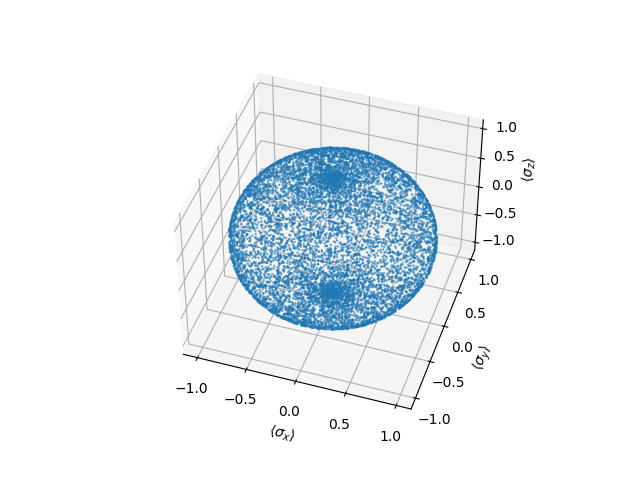
\includegraphics[width=0.6\textwidth]{method1_random_states_bloch_sphere.png}
		\caption{These ``random" states were generated with the method of generating random complex numbers with a gaussian distribution around the origin. Note the congregation of states around $\ket{+\bv{z}}$ and $\ket{-\bv{z}}$. This sampling is clearly not uniform across the bloch sphere.}
		\label{fig:method1_pure_bloch_sphere}
	\end{figure}
	
	\begin{figure}
		\centering
		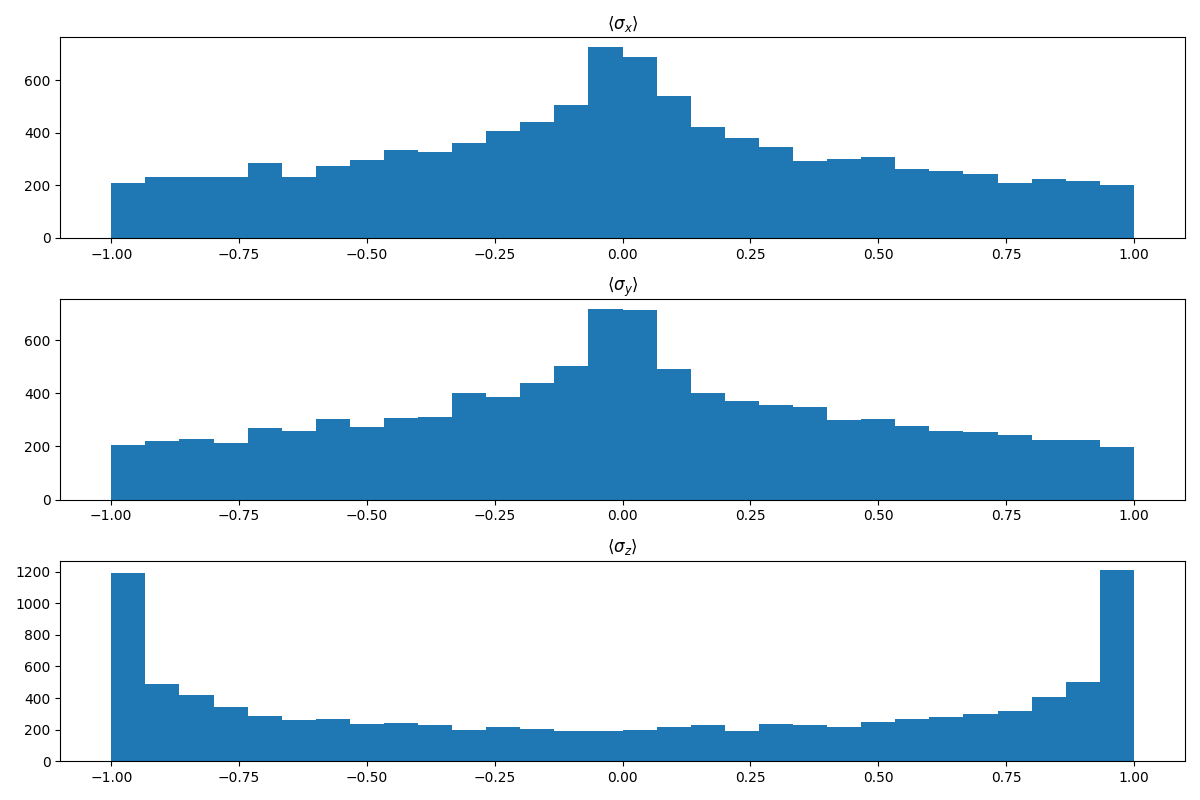
\includegraphics[width=0.6\textwidth]{method1_random_states_histograms.png}
		\caption{Histograms of the $x$, $y$, and $z$ positions for states generated with the second method (shown in \cref{fig:method1_pure_bloch_sphere}). With the same method of generating random complex numbers using a gaussian distribution about the origin, this plots histograms of the $\langle \sigma_z\rangle$, $\langle\sigma_y\rangle$, and $\langle\sigma_z\rangle$ for those states.}
		\label{fig:method1_pure_hists}
	\end{figure}
	
	The reason for this uneven distribution can be tracked down if you go ahead and calculate $\langle\sigma_x\rangle$, $\langle\sigma_y\rangle$ and $\langle\sigma_z\rangle$ for a state $\ket{\psi} = r_1e^{i\theta_1}\ket{+\bv{z}} + r_2e^{i\theta_2}\ket{-\bv{z}}$. You will obtain $\langle\sigma_x\rangle=2r_1r_2\cos\Delta\theta$, $\langle\sigma_y\rangle=2r_1r_2\sin\Delta\theta$ and $\langle\sigma_z\rangle=r_1^2-r_2^2$, which are clearly different distributions.

	\subsection{Random Probabilities (Good)}
	
	Instead of treating states as complex vectors in $\mathbb{C}^{2^n}$, this method begins with \textit{probabilities}. Namely, since the probability of $\ket{\psi}$ being in the basis state $\ket{e_j}$ is $|z_j|^2$, we begin with a fair probability distribution of probabilities $p_j$ that all sum to unity. Then the coefficients can be found as $z_j=\sqrt{p_j}e^{i\theta_j}$.
	
	This raises the question: ``what does it mean to find an even distribution of probabilities that sum to one?" This is a very important step that will come up again, and so the detailed answer to this question is given in \cref{apdx:random probability vectors}.

	\begin{figure}
		\centering
		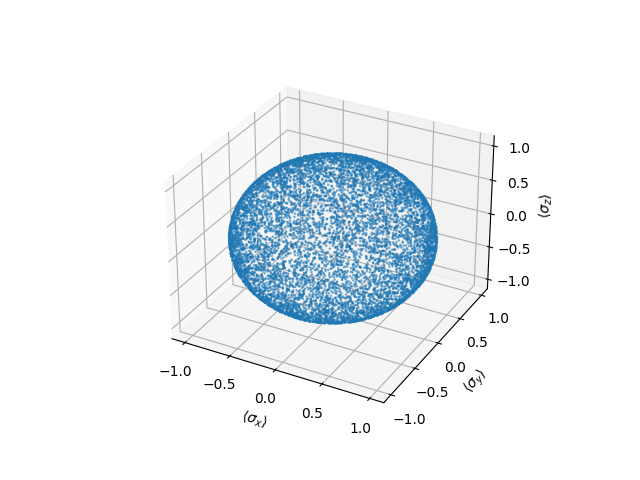
\includegraphics[width=0.6\textwidth]{method2_pure_bloch_sphere.png}
		\caption{10,000 random states were generated using the second method discussed, taking the square root of the probability vector.}
		\label{fig:method2_pure_bloch_sphere}
	\end{figure}
	\begin{figure}
		\centering
		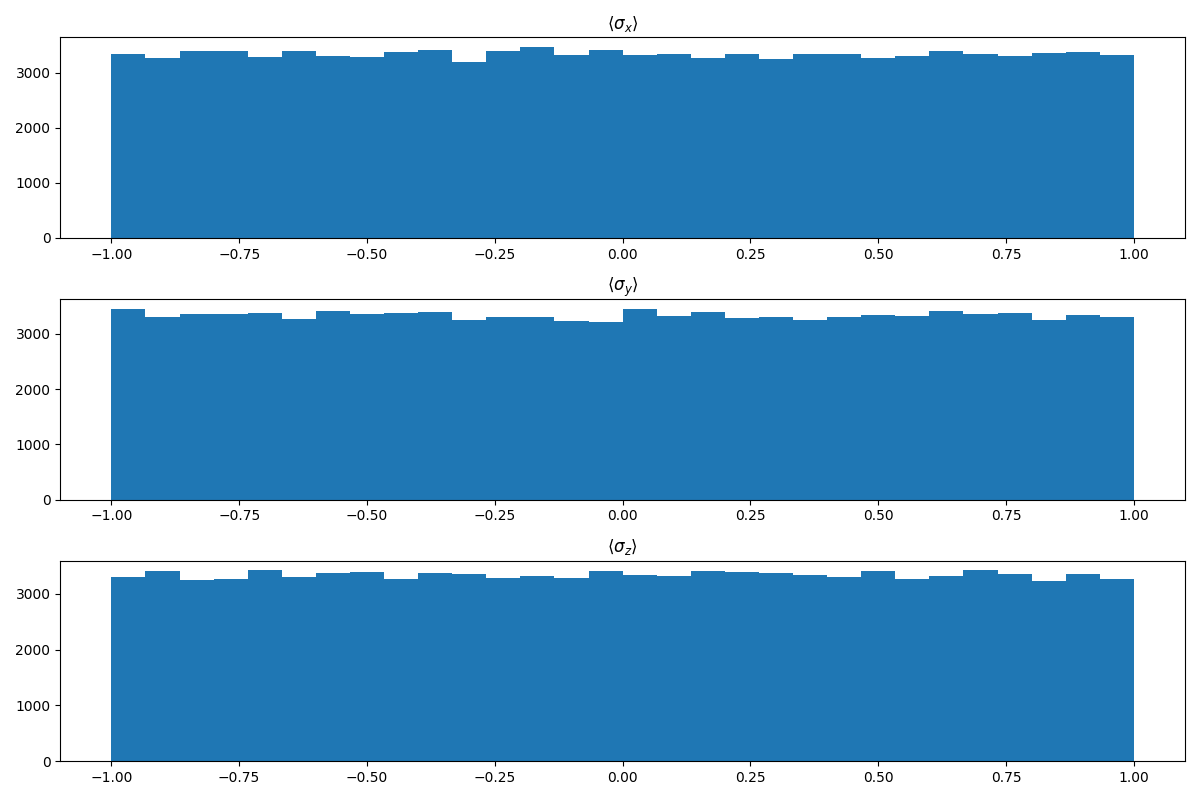
\includegraphics[width=0.6\textwidth]{method2_pure_histograms.png}
		\caption{Histograms of the $x$, $y$, and $z$ positions for states generated with the second method (shown in \cref{fig:method2_pure_bloch_sphere}). We've increased the sampling to 100,000 to emphasizes the uniformity of these distributions.}
		\label{fig:method2_pure_hists}
	\end{figure}
	
	\subsection{Double Gaussian}
	Another method that appears to be equally as effective as the probability method is an entirely gaussian distribution for both $\Re z_i$ and $\Im z_i$ before normalizing the vector. This means that the \texttt{random\_unit\_vector} function would then be
	\begin{verbatimtab}
		def random_unit_vector(dim):
			x = np.random.randn(dim) + 1j * np.random.randn(dim)
			x = x / np.linalg.norm(x)
    		return x
	\end{verbatimtab}
	
	Generation of plots like those in \cref{fig:method1_pure_bloch_sphere}-\ref{fig:method2_pure_hists} shows this method to be effectively equivalent to the probabilities method, but we will be sticking with the probabilities method for generating random states for the remainder of the exploration. I will not include plots for this generation method, as they look identical to the aforementioned plots, but code to generate these plots is available in the file \texttt{2-3.py}.
	
	\section{Random Mixed States}
	
	In this section, we dig into many methods for generating pseudo-random mixed states, discussing the pros and cons of each method.
	
	\subsection{Standard Method}
	% TODO: CITE STANDARD METHOD
	\subsection{Bloch-Parameterization Method}
	% TODO: CITE BLOCH PARAMETERIZATION
	\subsection{Pauli-Parameterization Method}
	\subsection{Trace Method}
	% TODO: CITE TRACE METHOD
	\subsection{N-Trace Method}
	\subsection{Over Parameterized Method}
	% TODO: CITE OVER PARAMETERIZED METHOD
	\section{Comparison and Conclusion}
	
	
	\appendix
	\section{Random Probability Vectors}\label{apdx:random probability vectors}
	
	A probability vector in this context is some vector $\bv{v}\in\mathbb{R}^m$ such that $\bv{v}\cdot\bv{1}=1$. This equation defines a plane of vectors that we wish to sample in some ``fair" way. To get a feel for what's going on here, we'll look at the generation of random probability vector in $\mathbb{R}^3$.
	
	\subsection{Normalizing a Gaussian or Uniform Distribution (Bad)}
	
	One way to approach this (and the first answer given on stack overflow) is to just use your distribution of choice, gaussian or uniform, to generate a vector of numbers, and then normalize that vector according to it's sum. Code for this might look like
	\begin{verbatimtab}
		def random_prob_vector(dim):
			x = np.dist(dim) # dist is your chosen distribution
			x = x / np.sum(x)
			return x
	\end{verbatimtab}
	However, this method causes issues. Let's look at the distribution of probability vectors in $\mathbb{R}^3$ that this method generates. Such distributions are shown in \cref{fig:prob_vecs_gauss} and \cref{fig:prob_vecs_uniform}, and both are noticeably uneven, in that there are larger concentrations of probability vectors in certain areas of the plane than others.
	
	The unevenness displayed in \cref{fig:prob_vecs_gauss} and \cref{fig:prob_vecs_uniform} is not necessarily a bad thing however, in fact, the correct probability distribution will also be ``uneven" in this manner of speaking. What matters more is \textit{how} they are uneven. I won't get too nitty-gritty here, but in higher dimensions when you have to pick random variables that sum to one, you are far more likely to get \textit{small} numbers than large ones. However, in both the distributions shown in the aforementioned figures, the clumping of probability vectors occurs near the center of the triangle, where the probabilities are relatively large and evenly spaced. You can justify why this would be for yourself by considering the space spanned by the original distribution, and how it projects down to this plane when we take the norm.
	
	\begin{figure}[ht]
		\centering
		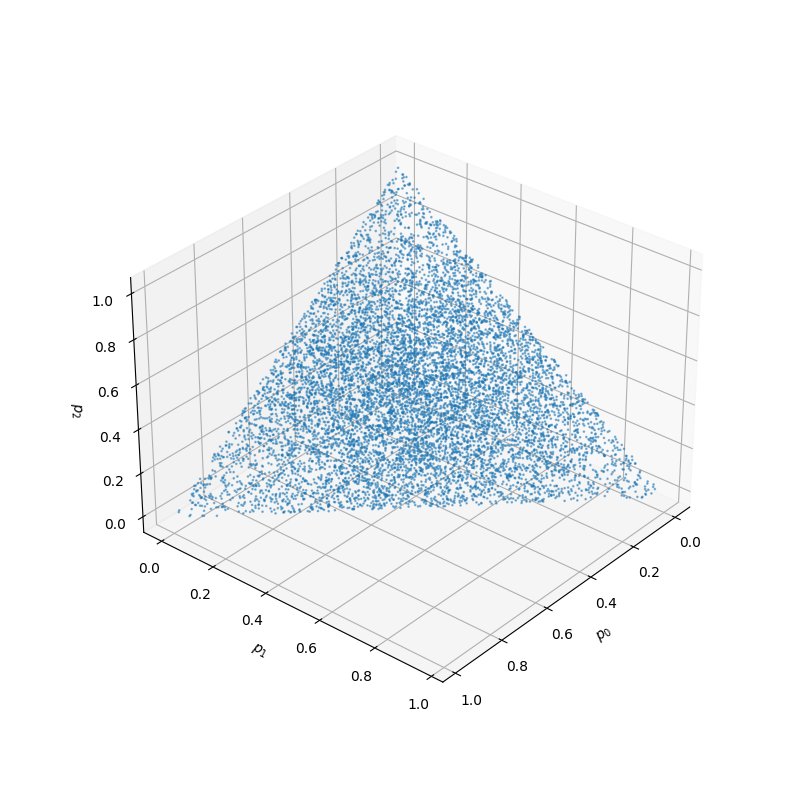
\includegraphics[width=0.6\textwidth]{prob_vecs_Gaussian.png}
		\caption{10,000 probability vectors generated by normalizing vectors from a \textbf{gaussian} distribution. Note the slight concentration of vectors towards the center of this triangle, as well as the more apparent lack of probability vectors near the vertices.}
		\label{fig:prob_vecs_gauss}
	\end{figure}
	\begin{figure}[ht]
		\centering
		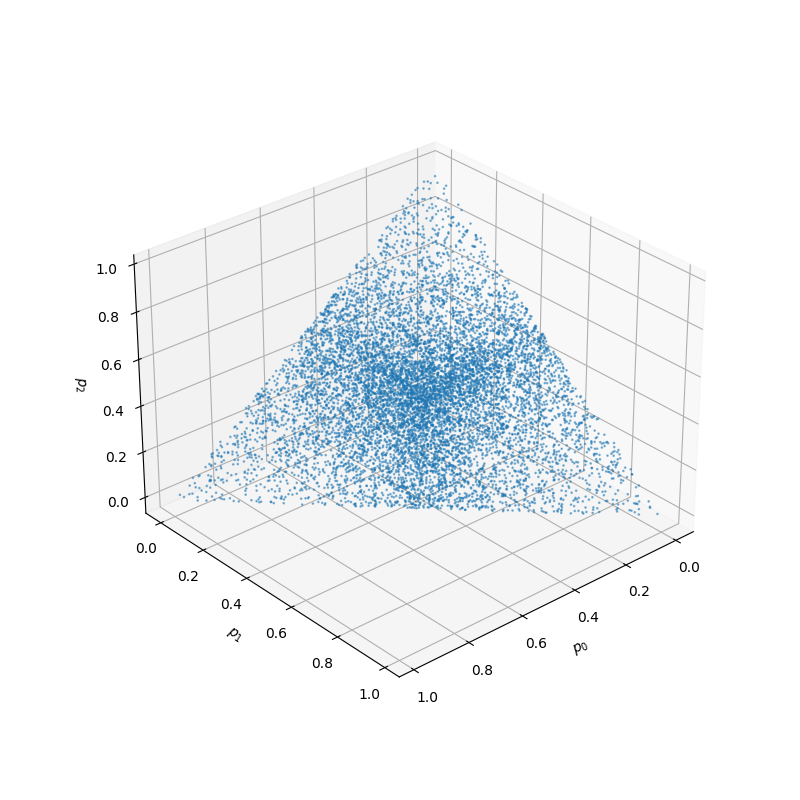
\includegraphics[width=0.6\textwidth]{prob_vecs_Uniform.png}
		\caption{10,000 probability vectors generated by normalizing vectors from a \textbf{uniform} distribution. Note the overwhelming concentration of probability vectors in the center of this triangle, as well as on the edges.}
		\label{fig:prob_vecs_uniform}
	\end{figure}
	
	\subsection{Correct Method}

	The correct method for random probability generation in higher dimensions is described in [CITE THE PAPER].
		% TODO: CITE THE PAPER
	First, we pick a random variable with a uniform distribution $p_1\in[0,1]$. Then for $p_2$ through $p_{m-1}$, you can use the following recursion relation to select the next probability with a uniform distribution
	\begin{equation*}
		p_i \in \left[0, 1 - \sum_{j=1}^{i-1} p_j\right]
	\end{equation*}
	Finally, you select $p_m = 1-\sum_{j=1}^{m-1} p_j$. This seems wildly unfair, for one thing you are virtually guaranteed for $p_m$ to be very small, however by applying a random permutation to the probabilities, we can achieve a totally fair distribution that also captures the fact that you are simply more likely to get smaller probabilities from a fair distribution. An illustrative plot of probability vectors generated with this method is shown in \cref{fig:prob_vecs_fair}.
	
	\begin{figure}[ht]
		\centering
		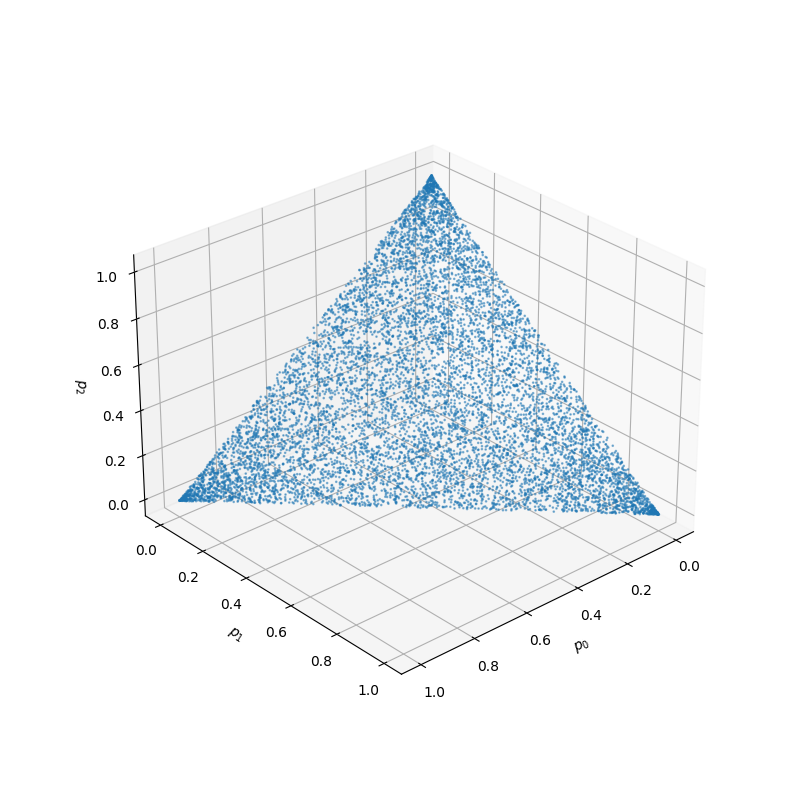
\includegraphics[width=0.6\textwidth]{prob_vecs_Fair.png}
		\caption{10,000 probability vectors generated using a ``fair" method. Note the concentrations at the vertices of the triangle, indicating that smaller probabilities are more likely here, as we would expect in three dimensions or larger.}
		\label{fig:prob_vecs_fair}
	\end{figure}

	
	
	
	
	
	
	
	
	
	
	
	
	
	
	
	
	
	

\end{document}